\documentclass[border=6pt]{standalone}
\usepackage[T1]{fontenc}\usepackage{lmodern}\usepackage{amsmath,bm}\usepackage{tikz}
\usetikzlibrary{positioning,fit,arrows.meta,calc,backgrounds,decorations.pathreplacing}
\newcommand{\K}{\bm{K}}\newcommand{\M}{\bm{M}}\newcommand{\C}{\bm{C}}\newcommand{\F}{\bm{F}}
\newcommand{\fea}{\texttt{fea\_engine}}\newcommand{\rom}{\texttt{rom\_engine}}
\newcommand{\cls}[1]{{\ttfamily\scriptsize #1}}
\begin{document}
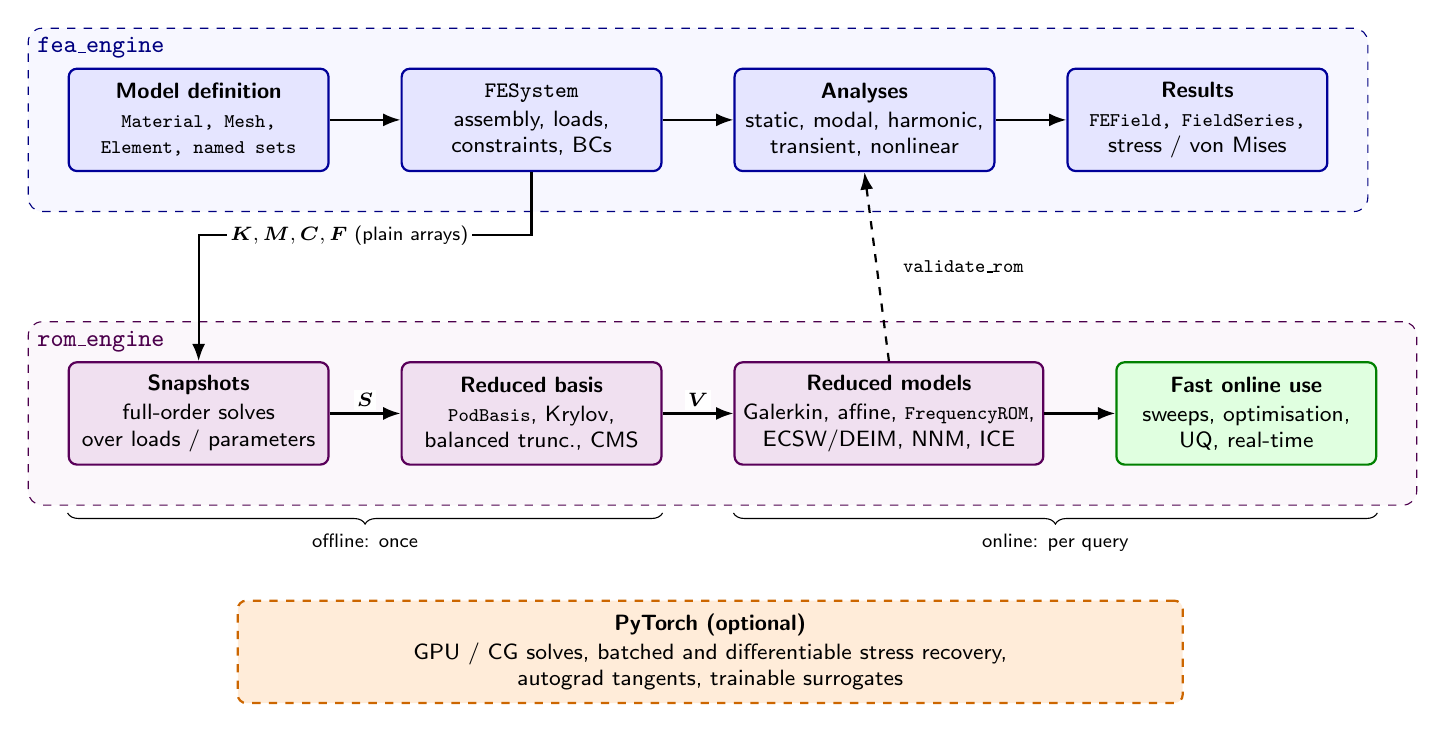
\begin{tikzpicture}[font=\sffamily\footnotesize, >=Latex,
  box/.style={draw, rounded corners=3pt, align=center, minimum height=13mm, minimum width=33mm, inner sep=3pt, thick},
  fe/.style={box, fill=blue!10, draw=blue!60!black},
  rm/.style={box, fill=violet!12, draw=violet!70!black},
  outb/.style={box, fill=green!12, draw=green!50!black},
  th/.style={box, fill=orange!15, draw=orange!80!black, dashed},
  flow/.style={-{Latex[length=2.2mm]}, thick},
  lab/.style={font=\sffamily\scriptsize, fill=white, inner sep=1.2pt}]
  % fea_engine lane
  \node[fe] (inp)  {\textbf{Model definition}\\[1pt]\cls{Material, Mesh,}\\\cls{Element, named sets}};
  \node[fe, right=9mm of inp] (sys) {\textbf{\texttt{FESystem}}\\[1pt]assembly, loads,\\constraints, BCs};
  \node[fe, right=9mm of sys] (ana) {\textbf{Analyses}\\[1pt]static, modal, harmonic,\\transient, nonlinear};
  \node[fe, right=9mm of ana] (res) {\textbf{Results}\\[1pt]\cls{FEField, FieldSeries,}\\stress / von Mises};
  % rom_engine lane
  \node[rm, below=24mm of inp] (snap) {\textbf{Snapshots}\\[1pt]full-order solves\\over loads / parameters};
  \node[rm, right=9mm of snap] (basis) {\textbf{Reduced basis}\\[1pt]\cls{PodBasis}, Krylov,\\balanced trunc., CMS};
  \node[rm, right=9mm of basis] (rom) {\textbf{Reduced models}\\[1pt]Galerkin, affine, \cls{FrequencyROM},\\ECSW/DEIM, NNM, ICE};
  \node[outb, right=9mm of rom] (on) {\textbf{Fast online use}\\[1pt]sweeps, optimisation,\\UQ, real-time};
  % lane backgrounds
  \begin{scope}[on background layer]
    \node[draw=blue!50!black, dashed, rounded corners=5pt, fill=blue!3, inner sep=5mm, fit=(inp)(sys)(ana)(res), label={[blue!50!black, font=\sffamily\small\bfseries, anchor=north west]north west:\fea{}}] (lane1) {};
    \node[draw=violet!60!black, dashed, rounded corners=5pt, fill=violet!3, inner sep=5mm, fit=(snap)(basis)(rom)(on), label={[violet!60!black, font=\sffamily\small\bfseries, anchor=north west]north west:\rom{}}] (lane2) {};
  \end{scope}
  % flows
  \draw[flow] (inp) -- (sys);
  \draw[flow] (sys) -- (ana);
  \draw[flow] (ana) -- (res);
  \draw[flow] (sys.south) |- ($(sys.south)+(0,-8mm)$) -| node[lab, pos=0.25, xshift=-2mm] {$\K,\M,\C,\F$ (plain arrays)} (snap.north);
  \draw[flow] (snap) -- node[lab, above=1pt] {$\bm S$} (basis);
  \draw[flow] (basis) -- node[lab, above=1pt] {$\bm V$} (rom);
  \draw[flow] (rom) -- (on);
  \draw[flow, dashed] (rom.north) -- node[lab, pos=0.5, xshift=11mm] {\cls{validate\_rom}} (ana.south);
  % offline / online brackets
  \draw[decorate, decoration={brace, amplitude=4pt, mirror}] ($(snap.south west)+(0,-6mm)$) -- node[below=4pt, font=\sffamily\scriptsize] {offline: once} ($(basis.south east)+(0,-6mm)$);
  \draw[decorate, decoration={brace, amplitude=4pt, mirror}] ($(rom.south west)+(0,-6mm)$) -- node[below=4pt, font=\sffamily\scriptsize] {online: per query} ($(on.south east)+(0,-6mm)$);
  % torch
  \node[th, below=17mm of $(basis.south)!0.5!(rom.south)$, minimum width=120mm] (torch) {\textbf{PyTorch (optional)}\\[1pt]GPU / CG solves, batched and differentiable stress recovery,\\autograd tangents, trainable surrogates};
\end{tikzpicture}
\end{document}
